
\documentclass[template=tabling,81pt,headonall]{azmoon}
\usepackage{xepersian}
\usepackage{amsfonts}
\usepackage{graphicx}
\graphicspath{ {./images/} }
\settextfont{Yas}
\setdigitfont{A Iranian Sans}
\usepackage{fontawesome5}

\printanswers
    \teacher{محمد صالح علی اکبری}
    \teachertitle{دبیر}
    \city{گناباد}
    \schooltitle{متوسطه دوره دوم}
    \school{شاهد امام (ره)}
    \grade{دهم}
    \branch{۱۵۱}
    \topic{ریاضی}
    \examdate{15/08/1402}
    \answertime{20 دقیقه}
    \begin{document}
	\begin{questions}
		\nointerlineskip%
		\vskip-\baselineskip
		\question{%
اگر $A = [-\dfrac{3}{2},\sqrt{5}]$ و $B = [\sqrt{3} , \dfrac{16}{3}]$ باشد. مجموعه $A\bigcup‌B$  شامل چند عدد صحیح است؟
    \begin{fourchoice}[4]\choice{$5$}
\choice{$6$}
\choice{$7$}
\choice{$8$}
\end{fourchoice}
    }
\question{%
اگر $n(A \bigcup B) = 20$، $n(A\bigcap B)=5$ و $2n(A) = 3n(B)$، مقدار $n(A)$ کدام است؟
    \begin{fourchoice}[4]\choice{$6$}
\choice{$9$}
\choice{$12$}
\choice{$15$}
\end{fourchoice}
    }
\question{%
در دنباله حسابی $a_{1} , a_{2} , ...$ حاصل $\dfrac{a_3}{a_2+a_4}+\dfrac{a_4}{a_3+a_5}+...+\dfrac{a_16}{a_{15}+a_{17}}$ چند است؟
    \begin{fourchoice}[4]\choice{$\dfrac{7}{2}$}
\choice{$\dfrac{13}{2}$}
\choice{$7.5$}
\choice{$7$}
\end{fourchoice}
    }
\question{%
در یک دنباله، جمله اول برابر ۴ و برای هر $n>1$، $\dfrac{a_n}{a_{n+1}}=2$. جمله دهم این دنباله کدام است؟
    \begin{fourchoice}[4]\choice{$\dfrac{1}{128}$}
\choice{$\dfrac{1}{64}$}
\choice{$1024$}
\choice{$2048$}
\end{fourchoice}
    }
\question{%
اگر x , y , 2 , z , t جمله‌های متوالی دنباله‌ای هندسی باشند، حاصل $\dfrac{x^2t^2}{yz}$ کدام است؟
    \begin{fourchoice}[4]\choice{$16$}
\choice{$2$}
\choice{$4$}
\choice{$8$}
\end{fourchoice}
    }
\question{%
اعداد $2^a$ ، $4\sqrt{2}$ ، $2^b$ سه چمله متوالی از یک دنباله هندسی اند. واسطه حسابی $a$ و $b$ کدام است؟
    \begin{fourchoice}[4]\choice{$\sqrt{2}$}
\choice{$1.5$}
\choice{$2$}
\choice{$2.5$}
\end{fourchoice}
    }
\question{%
در شکل زیر مربع‌های کوچک برابرند. مقدار $\tan\alpha$ کدام است؟ \\ 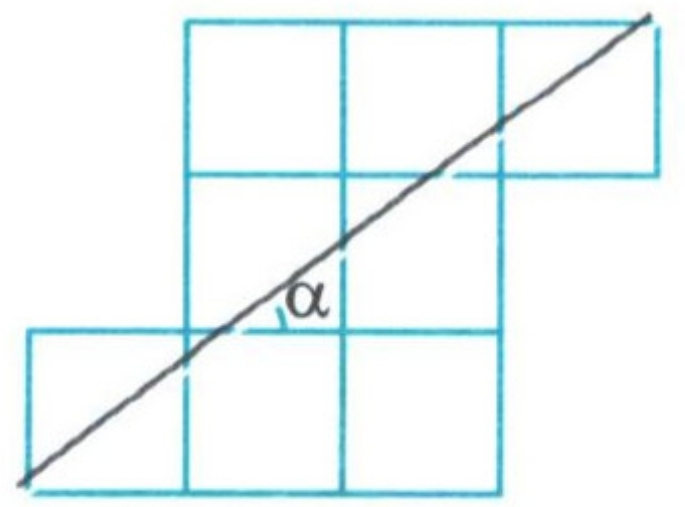
\includegraphics[scale = 0.18]{Screenshot_2023-11-06-06-32-43-456_cn.wps.moffice_eng-edit}
    \begin{fourchoice}[4]\choice{$\dfrac{2}{3}$}
\choice{$\dfrac{3}{2}$}
\choice{$\dfrac{4}{3}$}
\choice{$\dfrac{3}{4}$}
\end{fourchoice}
    }
\question{%
در شکل زیر طول ضلع مربع‌های کوچک برابر ۱ است. مقدار $\tan\alpha + \sin\alpha$ کدام است؟ \\ 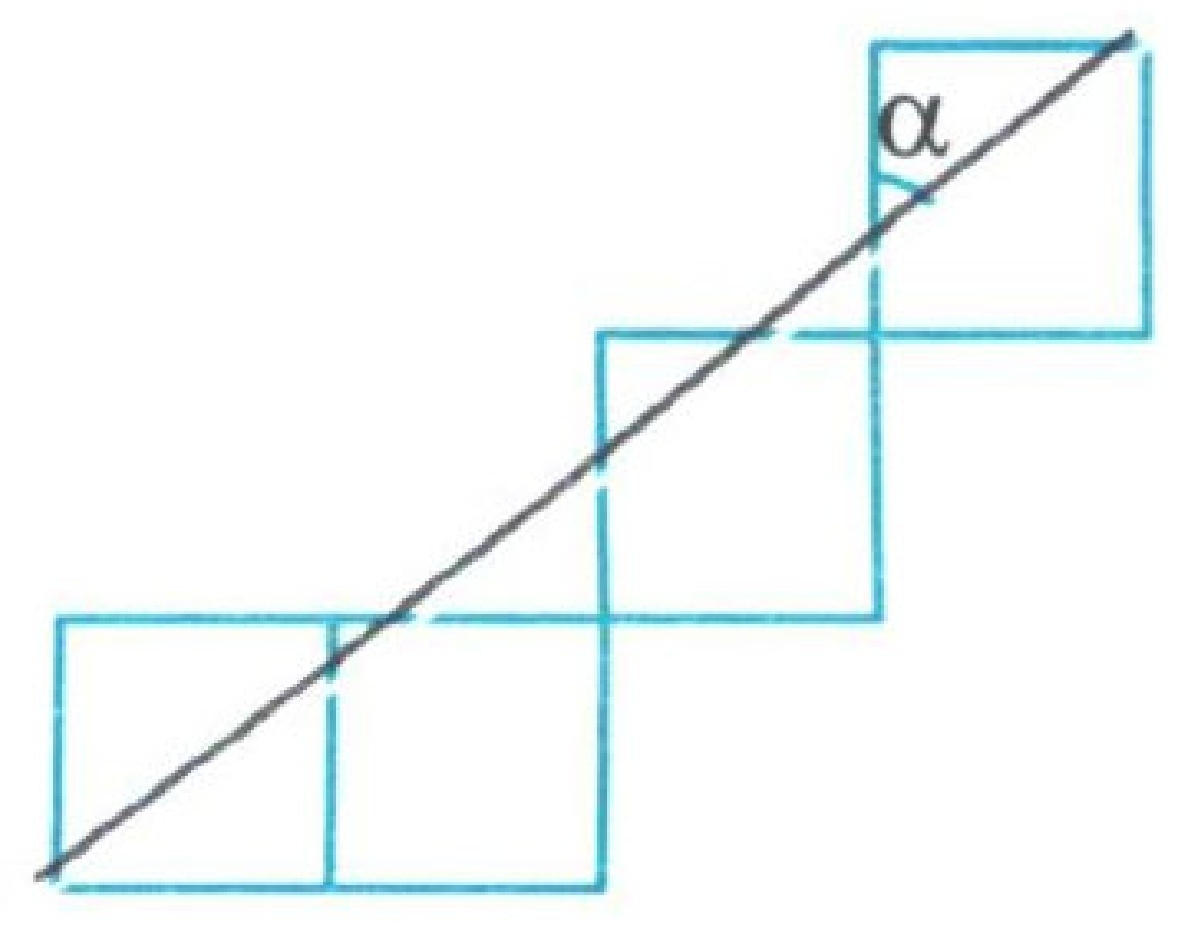
\includegraphics[scale = 0.08]{Screenshot_2023-11-06-06-40-47-663_cn.wps.moffice_eng-edit}
    \begin{fourchoice}[4]\choice{$\dfrac{34}{15}$}
\choice{$\dfrac{3}{15}$}
\choice{$\dfrac{32}{15}$}
\choice{$\dfrac{31}{15}$}
\end{fourchoice}
    }
\question{%
در شکل زیر $\tan \widehat{B} = \dfrac{1}{2}$ و $c-b=4$. مقدار $a$ کدام است؟ \\ 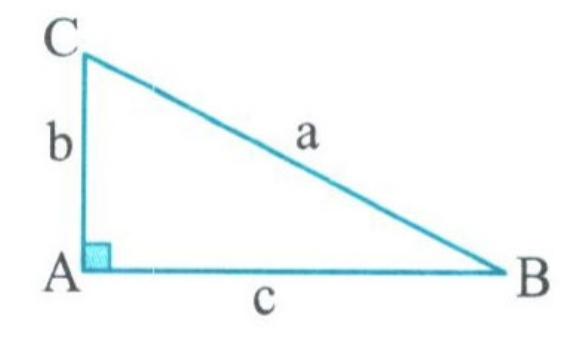
\includegraphics[scale = 0.3]{Screenshot_2023-11-06-06-44-17-910_cn.wps.moffice_eng-edit}
    \begin{fourchoice}[4]\choice{$2\sqrt{5}$}
\choice{$4\sqrt{5}$}
\choice{$3\sqrt{5}$}
\choice{$5\sqrt{5}$}
\end{fourchoice}
    }
\end{questions}
    \end{document}
    